\chapter{Planificación \label{sec:planificación}}
En este apartado se detallará la planificación del proyecto, indicando las diferentes fases del mismo, el desglose de las tareas que las componen y la duración de las mismas.

La planificación para el desarrollo del proyecto establece la duración del mismo en cinco meses, iniciándose este a principios de febrero y finalizando a mediados de junio, para la entrega del mismo y cumplir, así, la fecha de presentación del mismo establecida por la universidad Carlos III de Madrid.

\section{Fases de desarrollo}
En este apartado se describirán las fases en las que se ha dividido el trabajo y el tiempo de dedicado a ellas. Estas serán:

\begin{enumerate}
\item \textbf{Entendimiento del problema e identificación de las necesidades:}
El objetivo de esta fase es el análisis del problema para identificar las necesidades y pasos necesarios para solucionarlo. Se realiza el planteamiento del problema y se deciden las tecnologías a utilizar durante el proyecto y los entornos donde se realizará la implementación.

\begin{itemize}
\item Tiempo de ejecución: 7 días.
\end{itemize}

\clearpage
\item \textbf{Estudio de las tecnologías a utilizar:}
Se estudia el funcionamiento de las tecnologías a utilizar. Se analiza la documentación de \textit{Apache Spark} y se realizan diferentes cursos sobre la tecnología. Durante esta fase se analiza la inclusión de \textit{Apache Hadoop} y \textit{Apache Parquet}, que se acaban aceptando y se realiza su estudio.

\begin{itemize}
\item Tiempo de ejecución: 13 días.
\end{itemize}

\item \textbf{Diseño del sistema:}

Desarrollo teórico de las distintas posibilidades soluciones al problema planteado con las tecnologías establecidas. En esta parte, durante el análisis de las consultas a implementar, se añaden las modificaciones desarrolladas.

\begin{itemize}
\item Tiempo de ejecución: 15 días.
\end{itemize}

\item \textbf{Implementación del sistema en el entorno doméstico:}
Preparación del entorno de implantación y desarrollo del código necesario para desplegar el sistema en el entorno doméstico.
 
\begin{itemize}
\item Tiempo de ejecución: 17 días.
\end{itemize}

\item \textbf{Ejecución de pruebas y evaluación del entorno doméstico:}
En esta fase se produce la realización de la batería de pruebas establecidas para todos los componentes del sistema \textit{big data} en el entorno doméstico para ambas configuraciones. Tras la finalización se comprueban los resultados buscando errores y se repiten las pruebas necesarias.

\begin{itemize}
\item Tiempo de ejecución: 10 días.
\end{itemize}

\item \textbf{Implementación del sistema en el entorno universitario:}
En esta fase se produce el despliegue del sistema \textit{big data} para el entorno universitario. Al ser una adecuación del implementado en el doméstico, la principal tarea es la  del adaptación del sistema a los equipos.

\begin{itemize}
\item Tiempo de ejecución: 5 días.
\end{itemize}

\item \textbf{Ejecución de pruebas y evaluación del entorno universitario:}
En esta fase se produce la realización de la batería de pruebas establecidas para todos los componentes del sistema \textit{big data} en el entorno universitario para ambas configuraciones. Tras la finalización se comprueban los resultados buscando errores y se repiten las pruebas necesarias.

\begin{itemize}
\item Tiempo de ejecución: 7 días.
\end{itemize}

\item \textbf{Análisis de resultados:}
En este proceso se analizan todos los resultados obtenidos de las pruebas, se transforman los datos a un formato cómodo para su manipulación y se realizan las gráficas que se utilizarán en la memoria.

\begin{itemize}
\item Tiempo de ejecución: 9 días.
\end{itemize}

\item \textbf{Elaboración de la memoria:}
Documentación de todo el trabajo realizado en las fases anteriores.

\begin{itemize}
\item Tiempo de ejecución: 15 días.
\end{itemize}
\end{enumerate}

\section{Diagrama de fases de ejecución}
En la figura \ref{fig:ganttdelproyecto} podemos encontrar el diagrama Gantt del proyecto, donde se representan las fases nombradas anteriormente y su duración en el tiempo.

\begin{figure}[htp!]
\centering
\caption{Diagrama Gantt del proyecto}
\label{fig:ganttdelproyecto}
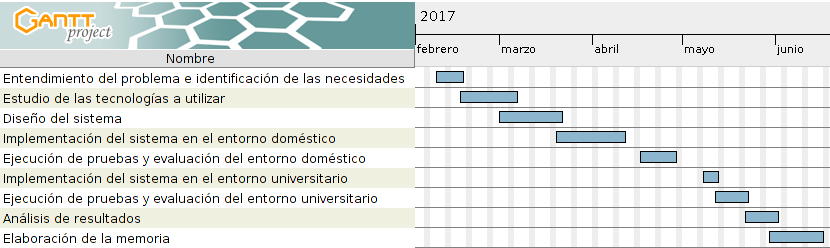
\includegraphics[scale=0.55]{graphics/gantDelProyecto}
\end{figure}